
%(BEGIN_QUESTION)
% Copyright 2006, Tony R. Kuphaldt, released under the Creative Commons Attribution License (v 1.0)
% This means you may do almost anything with this work of mine, so long as you give me proper credit

Some level switches use a vibrating rod or paddle to sense the presence of liquids or solids at a specific point.  Explain how such vibrating level switches work, in as much detail as you can.  Hint: sometimes these switches are known as {\it tuning fork} switches if they use two balanced paddles to sense the presence of liquid or solid material.

Also identify potential problems with this type of ``point-level'' detector caused by improper installation.

\underbar{file i00301}
%(END_QUESTION)





%(BEGIN_ANSWER)

These switches use an electronic circuit to vibrate the rod or paddle, then trigger their output signal upon sensing the dampening of that vibration caused by the presence of liquid or solid immersion.

Potential problems include:

$$\includegraphics[width=15.5cm]{i00301x01.eps}$$

%(END_ANSWER)





%(BEGIN_NOTES)


%INDEX% Switch, level: tuning fork

%(END_NOTES)


